\documentclass{llncs}
 
%% additional packages here
\usepackage[utf8]{inputenc}
\usepackage{eurosym}

\usepackage{graphicx}
\usepackage{float}

\usepackage[fleqn]{amsmath}
\usepackage{tabularx}
\usepackage{tabulary}
\usepackage{mathpartir}
\usepackage{amssymb}
\usepackage{subfiles}
%\usepackage{subcaption}

%% additional packages
\usepackage{color}
\usepackage{xcolor}
% shaded frameboxes
\usepackage{framed}
\definecolor{shadecolor}{rgb}{0.9,0.9,0.9}
\definecolor{Orange}{rgb}{1,0.5,0}

%\usepackage{mdframed}

\usepackage[pdftex]{hyperref}
\hypersetup{%
%pdftitle={\myTitle}, %
pdfauthor={blind submission}, %
%pdfkeywords={\programname},%
bookmarksnumbered, %
pdfstartview={c}, %
colorlinks,%
citecolor=black, %
filecolor=black, %
linkcolor=black, %
urlcolor=black}

\usepackage{mathtools}
\usepackage{cite}
\usepackage{epsfig}
\usepackage{epstopdf}
\usepackage{algorithm}
\usepackage{algorithmic}
\usepackage{caption}

%% Define authornote command for comments
\newcommand{\authornote}[2] {
    \begin{center}
        \framebox{
            \colorbox{yellow!40}{\begin{minipage}[t]{0.9\linewidth}
                \raggedright  \textbf{[#1]}~ \scriptsize #2 \normalsize
            \end{minipage}}
    }
    \end{center}
}

\newcommand{\structurenote}[2] {
    \begin{center}
        \framebox{
            \colorbox{purple!40}{\begin{minipage}[t]{0.9\linewidth}
                \raggedright  \textbf{[#1]}~ \scriptsize #2 \normalsize
            \end{minipage}}
    }
    \end{center}
}

% editing macros (and some cheats)

\newcommand{\lf}{\mbox{~}\\}
\newcommand{\todo}[1]{\textsf{\textbf{\textcolor{Orange}{[[#1]]}}}}
\newcommand{\todoreply}[1]{\textsf{\textbf{\textcolor{purple}{[[#1]]}}}}
\newcommand{\longpage}{\enlargethispage{\baselineskip}}

% % PM added to talk about PROV rels

\newcommand{\provGen}{\textit{provGen}}
\newcommand{\used}{\mathit{used}}
\newcommand{\wgby}{\mathit{genBy}}
\newcommand{\influence}{\mathit{wasInfluencedBy}}
\newcommand{\wdf}{\mathit{wasDerivedFrom}}
\newcommand{\waw}{\mathit{waw}}
\newcommand{\attrTo}{\mathit{wat}}
\newcommand{\wat}{\mathit{wat}}
\newcommand{\delegate}{\mathit{abo}}
\newcommand{\wasInfBy}{\mathit{wasInformedBy}}


%% Define program environment for code
\newenvironment{program}
{%
     \framed \scriptsize %
}
{%                
     \normalsize \endframed  %
}

\floatname{algorithm}{Procedure}
\renewcommand{\algorithmicrequire}{\textbf{Input:}}
\renewcommand{\algorithmicensure}{\textbf{Output:}}

%% Define subsection depth
\setcounter{secnumdepth}{3}
 



%opening
\title{PROV provenance representing the Twitter data model}

\author{Hugo Firth \and Paolo Missier}

\institute{School of Computing Science, Newcastle University, UK\\
           \{h.firth, paolo.missier\}@ncl.ac.uk
}

\begin{document}
\maketitle

\section{Introduction}
%
We describe a large synthetic corpus\footnote{https://github.com/provbench/Twitter-PROV} of PROV data, designed to represent the provenance of artefacts and interactions by users of the popular social network Twitter\footnote{https://twitter.com/}.
%
The data is topologically valid with respect to the PROV data model\cite{w3c-prov-dm}, and serialised using the PROV-N notation\cite{w3c-prov-dm}.
%
Table \ref{tab:corpusinformation} provides key information about the dataset itself.
%    
\begin{table}[H]
    \centering
    \caption{Information about the PROV corpus.}
    \label{tab:corpusinformation}
    \begin{tabular}{ | l | r | }
        \hline
        \, \textbf{Data format} \, &\, PROV-N \, \\ \hline
        \, \textbf{Data model} \, &\, PROV \, \\ \hline
        \, \textbf{Size on disk} \, &\, $\sim$ 250 Megabytes \, \\ \hline
        \, \textbf{Order} $\vert$V(G)$\vert$ \, &\, $\sim$ 1.5 Million \, \\ \hline
        \, \textbf{Size} $\vert$E(G)$\vert$ \, &\, $\sim$ 2 Million \, \\ \hline
    \end{tabular}
\end{table}
%
We elected to generate the described corpus, rather than collect it from some existing source, for several reasons:
%
\textit{1)} social networking data are not freely available, being of value to their respective service owners;
%
\textit{2)} the scale of social networking data precludes collecting more than a small sample for analysis or benchmarking purposes.
%
This ``through the keyhole'' approach results in an incomplete dataset, which significantly alters the type of analysis you can run against it.
% 
\section{Corpus creation}
%
Our provenance data was created using a modified version of the \provGen{}\footnote{http://prov-gen.com/} provenance generation tool, with carefully selected parameters designed to create a dataset which exhibited the same statistical characteristics as if it had been collected from Twitter itself.
%
These statistical characteristics of twitter data are determined using an informal report published by a social media analytics firm\footnote{http://www.beevolve.com/twitter-statistics/}.
%
They are not intended to be rigorous; merely provide the appearance of similarity.
%
The dataset represents the relationships and tweets of 1000 twitter users.
%
The number of followers per user is assigned randomly, according to a Gamma distribution\footnote{http://en.wikipedia.org/wiki/Gamma\_distribution}.
%
Figure \ref{fig:datamodel} depicts the anatomies of both the underlying Twitter data model being simulated, and the corresponding PROV representation.
%
\begin{figure}
    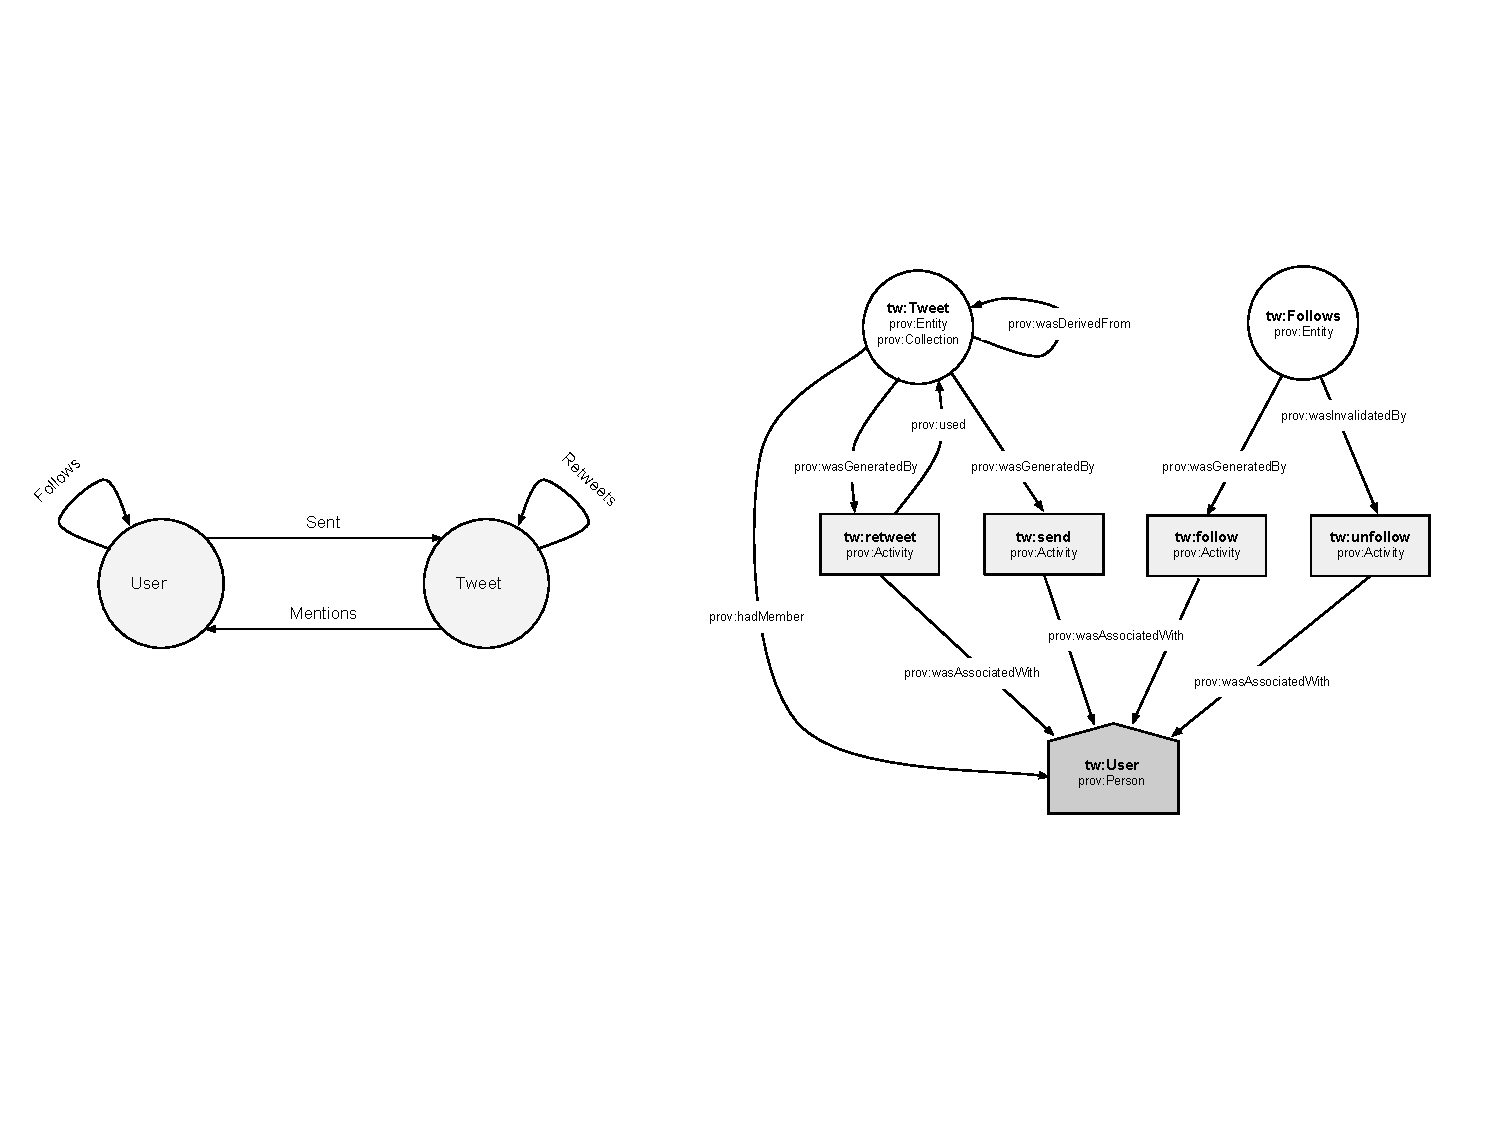
\includegraphics[width=1.1\textwidth]{figures/data_model}
    \caption{Twitter data model (left) and its PROV representation.}
    \label{fig:datamodel}
\end{figure}

%
\section{Motivation}
%
Traditional RDBMS, and the applications that make use of them, are primarily interested in ``shallow'' traversals, such as \textit{``Who are the friends of \ldots''} and \textit{``Which entries have x equal to y''}.
%
Provenance data, in part, models the dependencies of data.
%
Retrieving the dependency graph for any one piece of data may require an arbitrarily ``deep'' traversal.
%
Furthermore, existing RDBMS are often focused on frequent updates of stored data, which may require complex concurrency strategies to ensure the consistency of read operations. 
%
PROV data, on the other hand, is monotonic; write operations add new elements, rather than changing existing ones. 
%

%
We believe that the described dataset can be usefully applied to benchmarking the performance of systems designed to address these PROV specific characteristics, and supply a selection of sample queries to support this.
%
\section{Sample provenance queries}
%
\begin{enumerate}
    \item[Q1] \textit{What is the longest chain of derivations amongst Tweet Entities (retweets)?}
    
    This query might be used to measure the performance of a system at performing a large number of deep traversals of a dependency graph. 
    
    \item[Q2] \textit{What is the most influential Tweet Entity (most widely retweeted tweet)?}
    
    This query might be used to measure the performance of a system at performing broad, shallow, traversals of the type typically found in RDBMS and columnar stores.
     
    \item[Q3] \textit{What is the average number of unfollow Activities associated with a user Agent?}
    
    This query might be used to measure the performance at a system at performing aggregation tasks.
     
    \item[Q4] \textit{What is the great number of on-going Follows Entities attributed to a user Agent at any one time.}
    
    This query might be used to measure the performance of a system in providing answers about the historical state of a dataset.
    
\end{enumerate}
%
\section{Coverage of PROV}
%
We now address in more detail how nodes and relationships in the Twitter data model map to core PROV concepts.
%
\subsection{PROV Elements}
%
\begin{description}
  \item[Agent] \hfill \\
  Agents in the model are the Twitter users who are responsible for changes in the model state. In the described corpus, all activities are associated with an agent with type value \textit{prov:Person}.
  \item[Activity] \hfill \\
  Activities in the model represent actions taken by Twitter users and may take one of the following four forms: \textit{send}, \textit{retweet}, \textit{follow} and \textit{unfollow}. As with Agents this subclassing is achieved via the \textit{prov:type} extensibility point.
  \item[Entity] \hfill \\
  Entities in the model represent Tweets and Follow relationships. The latter has been reified in the PROV representation. Those Tweet entities which mention user agents have the type value \textit{prov:Collection} and have \textit{hadMember} relationships with mentioned agents.
\end{description}
%
\subsection{PROV Relations}
%
\begin{description}
  \item[used] \hfill \\
  The retweet activity \textit{uses} a Tweet entity.
  \item[wasGeneratedBy] \hfill \\
  The send activity \textit{generates} a Tweet entity. Further, a follow activity \textit{generates} a Follows entity.
  \item[wasDerivedFrom] \hfill \\
  A Tweet entity, generated by a retweet activity, is \textit{derived} from another Tweet entity.
  \item[wasAssociatedWith] \hfill \\
  All activities are \textit{associated} with user agents.
  \item[wasInvalidatedBy] \hfill \\
  A Follows entity is \textit{invalidated} by an unfollow activity. 
  \item[hadMember] \hfill \\
  A Tweet entity which mentions a user agent has that agent as a \textit{member}.
\end{description}
%
\section{Conclusions and further work}
%
In the submission of the described corpus to ProvBench we provide a single provenance dataset for benchmarking purposes.
%
The dataset is generated using specific parameters controlling, for example:
%
the statistical distribution of follower counts;
%
the correlation between variables such as Tweet count and follow count;
%
and the base probability of certain events (such as one user unfollowing another).
%
Given these facts, we can usefully continue to produce further Twitter-PROV datasets.
%
Each generation varying individual parameters in an attempt to quantify the impact of data with different statistical characteristics, upon provenance management systems.
%

Finally, the use of timestamps in the dataset is restricted to \textit{follow} \& \textit{unfollow} activities. This is a result of the complexity involved in calculating correlations between Tweets and Follow relationships over time. However, technical issues not withstanding, this could prove a useful addition to the datasets, and should form the basis for further work.

\bibliographystyle{plain}
\bibliography{provbench}

\end{document}  
